\begin{figure*}[h]
    \centering
    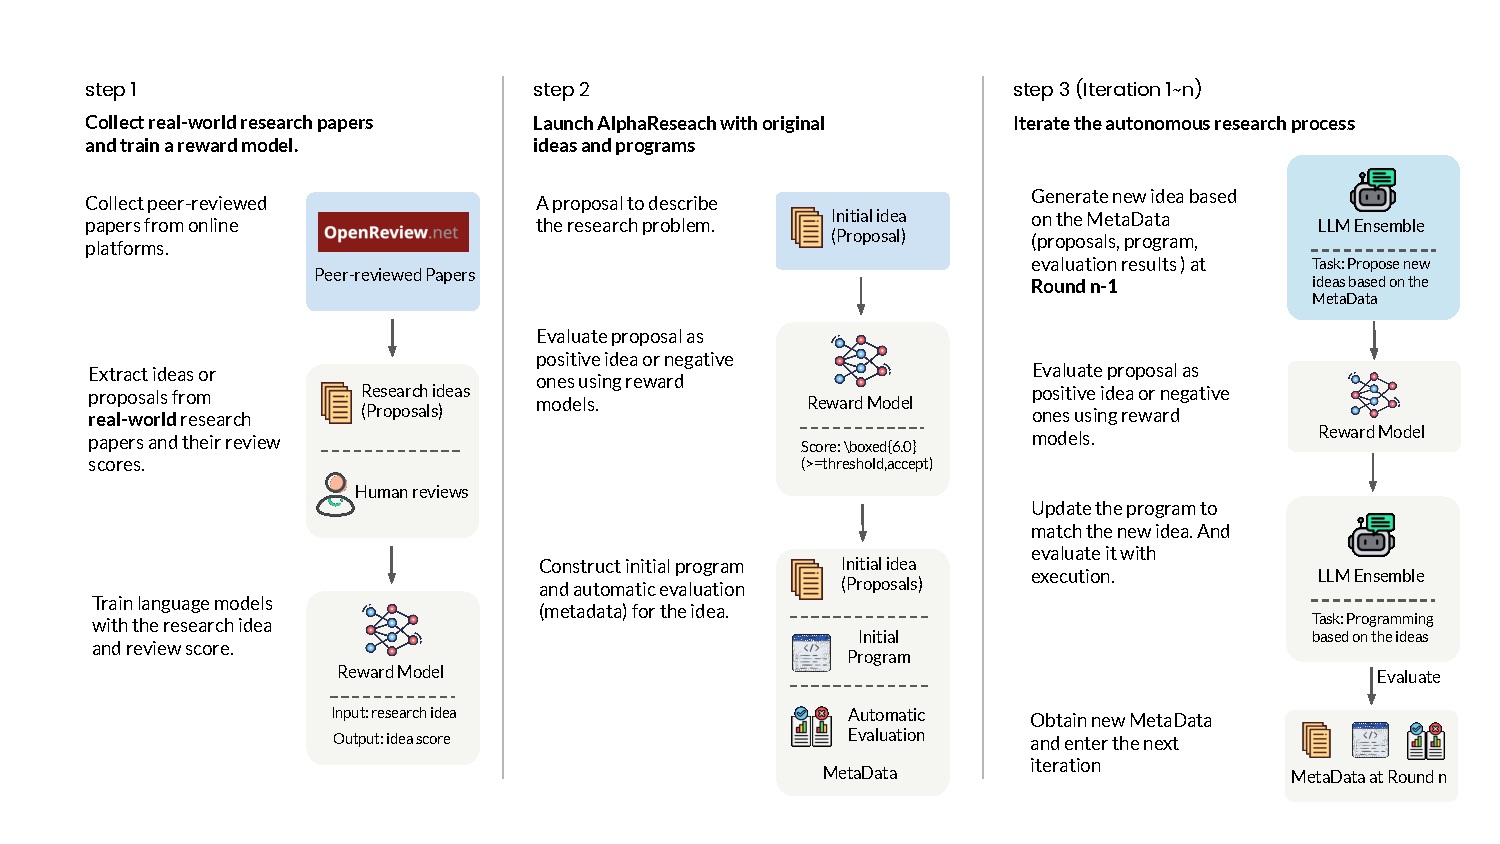
\includegraphics[width=0.95\linewidth]{doc/figures/alpharesearch-overview.pdf} 
    \caption{
    % The launch of AlphaResearch contains two steps: (1) Train reward models with real-world peer-reviewed records. (2) Prepare initial research proposals, initial programs and evalution program. It will then iteratively refine the research proposals and programs (3).
    Overview of AlphaResearch. This system accelerates discovery process with interleaved idea generation and program generation, where it get reward from peer-review model and program execution.
    }
    \label{fig:overview}

\end{figure*}

\section{Introduction}
Recent progress has shown that sophisticated coding agent scaffolds \citep{yang2024swe} could help frontier LLMs~\citep{gpt5, comanici2025gemini} achieve expert-level performance in end-to-end coding problems (e.g., modify the code to pass the test cases in sandbox~\citep{jimenez2024swebench}).
% But for open-ended coding problems where the final results (end-points) are unpredictable, end-to-end coding agents often 
However, for open-ended coding problems where the target endpoint (i.e., the optimal implementation) is left underspecified, end-to-end coding agents often struggle to converge on the best possible solution with just a few attempts.

AlphaEvolve~\citep{novikov2025alphaevolve} shows that scaling the number of agent attempts can reveal an emerging ability to derive stronger solutions from suboptimal prior results. 
% However, it relies on a "brute-force search" system: each new attempt is generated by sampling a previous attempt from the program database, and this process repeats until a preset iteration limit is reached.
% This leads to a significant increase in runtime for validating attempts, which naturally raises the following research question:
However, its brute-force search process repeatedly samples new attempts from a program database until a preset iteration limit is reached, substantially increasing validation cost.
This raises a key question:
\emph{Can we accelerate new algorithm discovery by reducing ineffective attempts?}

ShinkaEvolve~\citep{lange2025shinkaevolve} advances this direction by introducing a more sample-efficient evolutionary framework for open-ended program evolution. Specifically, it filters out redundant or minimally changed edits before expensive validation using a novelty rejection-sampling mechanism that combines embedding-based code similarity with an LLM-based novelty judge. This improves exploration efficiency relative to pure brute-force sampling, but important limitations remain. Embedding-based similarity thresholds can miss semantically meaningful changes or, conversely, fail to detect subtle redundancies. In addition, LLM-based novelty judgments are inherently unreliable because there is little high-quality training data explicitly annotated for program novelty in open-ended evolutionary search. As a result, general-purpose LLMs may rely on superficial cues and produce judgments that diverge from expert assessments of functional improvement, algorithmic originality, or non-trivial semantic change~\citep{zheng2023judging, szymanski2025limitations, lin2025evaluating}. These limitations motivate the need for more robust and efficient mechanisms for balancing exploration and exploitation in scalable algorithm discovery systems.
% ShinkaEvolve~\citep{lange2025shinkaevolve} takes an important step toward addressing this challenge by introducing a more sample-efficient evolutionary framework for open-ended program evolution. In particular, it employs a code novelty rejection-sampling mechanism based on embedding similarity of code snippets combined with an LLM-as-a-novelty-judge assessment to filter out redundant or minimally different modifications before expensive validation. 
% While this approach improves exploration efficiency and reduces wasted evaluations compared to pure brute-force sampling, it still faces notable limitations. The embedding-based similarity threshold can be overly insensitive to semantically meaningful differences, occasionally rejecting promising variants or failing to catch subtle redundancies. More critically, the reliance on LLM-as-a-judge for novelty assessment introduces fundamental challenges stemming from the scarcity of high-quality training corpora specifically annotated for scoring program novelty. General-purpose LLMs are not fine-tuned on large-scale, expert-labeled datasets that capture nuanced notions of code novelty, such as functional improvements, algorithmic originality, or non-trivial semantic divergence beyond syntactic changes, in the context of open-ended evolutionary search. Instead, they inherit biases and blind spots from broad pre-training data, leading to inconsistent, superficial, or unreliable novelty judgments that diverge from expert human assessments of true algorithmic innovation~\citep{zheng2023judging, szymanski2025limitations, lin2025evaluating}. This lack of domain-specific supervision undermines judgment reliability, thereby limiting the sample-efficiency gains in practice. These issues highlight the need for more robust and efficient mechanisms to balance exploration and exploitation in scalable algorithm discovery systems.

% For example, these systems could converge on technically correct but scientifically uninteresting or less impactful solutions—code that executes successfully yet offers no advancement over existing methods. Conversely, idea-generation systems evaluated purely by LLM judges can propose innovative concepts that prove computationally infeasible or violate problem constraints when implemented.
% % \ac{What is the limitation of AlphaEvolve that we aim to address?}
% The absence of real-world research environment rewards in execution-based agents and execution-based reward in idea-generation systems renders the discovery of new knowledge 
% and algorithms challenging for current autonomous research agents \citep{Tian2024SciCodeAR}.



% While LLMs excel at processing and reasoning on problems that are within the boundary of existing human knowledge~\citep{wang2024mmlupro, phan2025humanity},

% their capacity for independent discovery from existing human knowledge still remains a question of paramount importance~\citep{novikov2025alphaevolve}. 




% Previous studies demonstrate that LLMs can generate novel ideas at a human expert level~\citep{si2024can, wang2024scimon}. However, the outcome evaluation of LLM-generated research ideas still struggles with biased verification methods~\citep{ye2024justice} that constrain the exploration of out-of-boundary machine knowledge, such as LLM-as-a-judge~\citep{lu2024ai}, where misaligned LLMs are used to evaluate fresh ideas and inevitably favor solutions within existing knowledge boundaries. Furthermore, the ideation–execution gap \citep{si2025ideation} between generating and executing new ideas also hinders models from producing advanced research outcomes.
% \ac{We should clarify how previous work uses LLM-as-judge for research loops. Is it primarily a feedback loop where the judge guides model improvement? If so, is the limitation that because LLM-as-judge operates within existing knowledge boundaries, it cannot push models beyond known knowledge?}
% \ac{Also mention that there is a gap between generating ideas and ideas that are actually executable to tangible outcomes: https://arxiv.org/pdf/2506.20803}
% AlphaEvolve \citep{novikov2025alphaevolve} introduces an evolutionary coding agent that could tackle open scientific problems with program-based verification.
% % \ac{What is the limitation of AlphaEvolve that we aim to address?}
% However, the absence of real-world research environment rewards in coding-only agents~\citep{Tian2024SciCodeAR} renders the discovery of out-of-boundary knowledge and algorithms challenging for current autonomous research agents.


% \ac{I'm not sure if we can quantify the ``out-of-boundary'' knowledge well. Make this a softer claim or maybe use another term than out-of-boundary knowledge.} 
% and algorithms challenging for current autonomous research agents \citep{Tian2024SciCodeAR}.


% discovering out-of-boundary knowledge and algorithms with a research agent still remains challenging for current LLMs.
% \yilun{cite AlphaEvolve in first or second paragraph?}

% In this paper, we introduce \textbf{\ours}, an autonomous research agent designed to discover new advanced algorithms by ensembling LLMs with a suite of research skills, including idea generation, code implementation, and iterative optimization.
% To combine the feasibility and innovation of the algorithm discovery
% process, we construct a dual environment, where novel algorithms are forged by the simulated 
% real-world peer-reviewed environment and execution-based verification  \citep{Tian2024SciCodeAR}. Specifically, we (1) train a reward model \textbf{AlphaResearch-RM-7B} with real-world peer-reviewed records to simulate the real-world peer review environment, addressing the limitation of prior coding-only approaches that lack real-world research feedback, and use it to score the fresh ideas generated by LLMs.
% % \ac{This is a good contribution, but we don't motivate it well (e.g., what gap exists in current approaches) in the previous paragraph. } 
% (2) construct an automatic program-based verifiable environment that executes these ideas with an interpreter.
% This dual environment facilitates a rigorous algorithm discovery process for autonomous research agents. 
% \kaiyue{would this be better?: Specifically, we (1) train a reward model \textbf{AlphaResearch-RM-7B} with real-world peer-reviewed records, addressing the limitation of prior coding-only approaches that lack real-world research feedback, and use it to score the fresh ideas generated by LLMs;
% (2) construct an automatic program-based verifiable environment that executes these ideas with an interpreter.}

% AlphaResearch discovers new algorithms by iteratively running the following steps: (i) proposing new research ideas, (ii) programming based on strong ideas, and (iii) optimizing the proposals for better algorithms. The commencement of each iteration in AlphaResearch mandates an LLM's creation of a new idea informed by previous research findings. After obtaining a fresh idea, AlphaResearch-RM will preserve the positive ideas as candidates and discard the negative ones.
% % \ac{Unclear. Do we retrain the RM based on positive ideas? If so a ``based on'' might be missing in the previous sentence. I think what you mean is score not retrain?}
% Those positive ideas are then implemented into executable programs by coding agents ensembled with LLMs. 
% The program is subjected to rigorous code execution and automatic evaluation, a process previously demonstrated to be highly effective in mitigating incorrect suggestions often observed from LLMs \citep{Tian2024SciCodeAR}.
% ========================
In this paper, we introduce \textbf{\ours}, an autonomous research-based coding agent that could reduce ineffective attempts and accelerate new algorithm discovery by interacting with real-world peer-review  environments.
As shown in \autoref{fig:overview} and \autoref{tab:compofagent},  AlphaResearch construct a novel dual research-based environment, where the research ideas proposed by LLMs could be judged by a simulated real-world peer-review environment and then attempt by code sandbox.
Specifically, we (1) train a reward model \textbf{AlphaResearch-RM-7B} with real-world peer-review records, addressing the limitation of prior coding-only approaches that lack real-world research feedback, and use it to score the fresh ideas generated by LLMs;
\begin{table}[!t]
    \centering
    \small
    \begin{tabular}{l|ccc}
    \toprule
\multirow{2}{*}{\textbf{Agent}} 
    & \multicolumn{3}{c}{\textbf{Environments}} \\
    & Sandbox                  & Database & Peer-review Feedback \\
    \midrule
        SWE-agent \citep{yang2024swe} & \color{darkgreen}\ding{52} & \color{red}\ding{56} & \color{red}\ding{56} \\
        AlphaEvolve \citep{novikov2025alphaevolve} & \color{darkgreen}\ding{52} & \color{darkgreen}\ding{52} & \color{red}\ding{56} \\
        ShinkaEvolve \citep{lange2025shinkaevolve} & \color{darkgreen}\ding{52} & \color{darkgreen}\ding{52} & \color{red}\ding{56} \\
        AlphaResearch (ours) & \color{darkgreen}\ding{52} & \color{darkgreen}\ding{52} & \color{darkgreen}\ding{52} \\
      \bottomrule
    \end{tabular}
    \caption{Comparison of AlphaResearch and other agents.}
    \label{tab:compofagent}
\end{table}
% Specifically, we (1) train a reward model \textbf{AlphaResearch-RM-7B} with real-world peer-reviewed records to simulate the real-world peer review environment and score the fresh ideas generated by LLMs 
% \ac{This is a good contribution, but we don't motivate it well (e.g., what gap exists in current approaches) in the previous paragraph. } 
(2) construct an automatic program-based verifiable environment that executes these ideas with an interpreter.
This dual environment facilitates a rigorous algorithm discovery process for autonomous research agents. As illustrated in \autoref{fig:overview}, AlphaResearch discovers new algorithms by iteratively running the following steps: (i) proposing new research ideas, (ii) verify the ideas in the dual research-based environment, and (iii) optimizing the proposals for higher reward from the environment. 
The synergy between an iterative real-world peer review environment and program-based verification empowers AlphaResearch to continuously explore novel research ideas and verify the attempts via less program execution. 

% \ac{we need to motivate why we create this and why existing resources and datasets (e.g., those used in AlphaEvolve) are not sufficient to evaluate AlphaResearch}
To facilitate the comparison between AlphaResearch and other baselines (e.g., AlphaEvolve and ShinkaEvolve), we collect 8 open-ended research problems and their best-of-human records \textbf{\dataset} and simulate an algorithm discovery \textbf{comp}etition between AlphaResearch and other agents for discovery.
% \ac{Why we name it AlphaResearchComp? (Comp part is unclear).}
% \ac{Need to add one more sentence to describe what is special about this dataset, what are the composition of problems, etc.}
Our experimental results show that AlphaResearch achieves a score of 2.939 on the \emph{“Packing Circles (n=32)”} problem, surpassing the previous results obtained by AlphaEvolve (see \autoref{app:examples}). 
Furthermore, compared with ShinkaEvolve, which adopts code-novelty-based rejection sampling, AlphaResearch demonstrates faster convergence to higher-performing programs on three out of four open-ended problems. This highlights the effectiveness of the peer-review environment constructed in AlphaResearch. 
We also analyze the advantages and remaining challenges of autonomous research agents for knowledge discovery, providing insights for future work.
% Our results demonstrate that AlphaResearch surpasses human researchers on two problems but fails on the other six. 

% In the competition with OpenEvolve~\citep{openevolve}, an open-sourced implementation of AlphaEvolve,
% AlphaResearch optimizes the result of \emph{``Packing Circles (n=32)''} problem to 2.939, where the goal is to pack $n$ disjoint circles inside
% a unit square so as to maximize the sum of their radii, surpassing the results of best-of-human and previous SoTA results achieved by AlphaEvolve (as shown in \autoref{app:examples}).
% Furthermore, compared to AlphaEvolve, AlphaResearch's discovery process exhibits better and faster convergence on other six competitions. 
% \ac{These results are not very meaningful if people don't understand the metric and the problem. Maybe don't go into details of the numbers here.}
% \ac{we need to also add description saying that while it works on 2 problems, it still fails on 6 of the other problems, showing that there is large room for future work. And then say that we perform careful analysis to provide useful insights...}


To summarize, our key contributions are the following: 
\begin{itemize}[leftmargin=*]
\itemsep0em
    \item We introduce AlphaResearch, a novel autonomous research agent designed to accelerate the discovery of new algorithms by synergistically combining idea generation, code implementation, and verification in a dual environment of simulated peer review and executable program validation.
    \item We benchmark AlphaResearch with other agents for discovery across diverse verifiable problems to showcase the advantages of AlphaResearch in reducing ineffective attempts and accelerating new algorithm discovery.
    \item We present systematic ablations and analysis to understand the importance of incorporating peer-review environments into LLM-based autonomous discovery system.
\end{itemize}
